% Author: Anastasiia Samoilova <xsamoi00@stud.fit.vutbr.cz>
% Author: Maksim Dubrovin <xdubro01@stud.fit.vutbr.cz>
% Author: Ilya Volkov <xvolk02@stud.fit.vutbr.cz>
% Author: Anastasiia Mironova <xmiron05@stud.fit.vutbr.cz>


\documentclass[a4paper, 11pt]{article}


\usepackage[czech]{babel}
\usepackage[utf8]{inputenc}
\usepackage[left=2cm, top=3cm, text={17cm, 24cm}]{geometry}
\usepackage{times}
\usepackage{verbatim}
\usepackage{enumitem}
\usepackage{graphicx} % vkládání obrázků
\usepackage[unicode]{hyperref}


\newcommand{\RNum}[1]{\uppercase\expandafter{\romannumeral #1\relax}} % makro na sázení římských čísel


\begin{document}


	%%%%%%%%%%%%%%%%%%%%%%%%%%%%%%%% Titulní stránka %%%%%%%%%%%%%%%%%%%%%%%%%%%%%%%%
	\begin{titlepage}
		\begin{center}
			
\includegraphics[width=0.9\linewidth]{FIT_LOGO.pdf} \\

			\vspace{\stretch{0.382}}

			\Huge{Projektová dokumentace} \\
			\LARGE{\textbf{Implementace překladače imperativního jazyka IFJ23}} \\
			\Large{Tým xdubro01}
			\vspace{\stretch{0.618}}
		\end{center}

		\begin{minipage}{0.4 \textwidth}
			{\Large \today}
		\end{minipage}
		\hfill
		\begin{minipage}[r]{0.6 \textwidth}
			\Large
			\begin{tabular}{l l l}
				\textbf{Maksim Dubrovin} & \textbf{(xdubro01)} & \quad 25\,\% \\
				Anastasiia Samoilova & (xsamoi00) & \quad 25\,\% \\
				Ilya Volkov & (xvolk02) & \quad 25\,\% \\
				Anastasiia Mironova & (xmiron05) & \quad 25\,\% \\
			\end{tabular}
		\end{minipage}
	\end{titlepage}



	%%%%%%%%%%%%%%%%%%%%%%%%%%%%%%%% Obsah %%%%%%%%%%%%%%%%%%%%%%%%%%%%%%%%
	\pagenumbering{roman}
	\setcounter{page}{1}
	\tableofcontents
	\clearpage



	%%%%%%%%%%%%%%%%%%%%%%%%%%%%%%%% Úvod %%%%%%%%%%%%%%%%%%%%%%%%%%%%%%%%
	\pagenumbering{arabic}
	\setcounter{page}{1}

	\section{Úvod}
         Tento dokument byl vytvořen jako dokumentace pro projekt IFJ, popisující metody implementace všech komponent kompilátoru i problémy během uvedené implementace.

	Cílem projektu je vytvořit program v~jazyce~C, který načte zdrojový kód zapsaný ve zdrojovém jazyce IFJ23
    a přeloží jej do cílového jazyka IFJcode23

	%%%%%%%%%%%%%%%%%%%%%%%%%%%%%%%% Implementace %%%%%%%%%%%%%%%%%%%%%%%%%%%%%%%%
	\section{Implementace}
        Projekt jsme udělali z několika námi realizovaných částí, které jsou v této kapitole. \\
        \\
	Kompilátor se skládá z následujících komponent: \\
        1. Lexikální analyzátor \\
        2. Syntaktický analyzátor \\
        3. Sémantický analyzátor  \\
        4. Generátor kódu \\
        \\
        Vstupní kód je zpracován každou komponentou ve stejném pořadí, v jakém je zapsán
        výše uvedený seznam.


	\subsection{Lexikální analýza}

        Lexikální analýza probíhá v \texttt{scanner.c}, tento soubor obsahuje implementaci skeneru.
        Skener čte vstupní zdrojový kód znak po znaku, přeskakuje prázdné místo a komentáře a identifikuje různé tokeny, jako jsou čísla, řetězce, identifikátory a symboly. V tomto souboru používáme pomocné funkce, které jsou implementovány v souborech \texttt{str.c} a \texttt{token.c}.
        Funkce \textbf{scanToken} v \texttt{scanner.c} je jádrem skeneru, který je zodpovědný za identifikaci a vytváření tokenů na základě vstupních znaků.
        

        \subsubsection{ Podstata a souvislost procesu práce v souborech }
        V souboru \texttt{token.c} používáme funkce, které pomáhají při zpracování tokenů. Poskytované funkce umožňují vytváření, načítání a mazání tokenů a také dynamickou změnu velikosti tak, aby vyhovovala proměnné délce seznamu.\\
        \\
        V souboru \texttt{str.c} funkce poskytují základní řetězcové operace potřebné při lexikální analýze a dalších částech kompilátoru. Zpracovávají výpočet délky řetězce, porovnání řetězců, kopírování řetězců a transformace, jako je přidání znaménka mínus do lexému tokenu.\\
        \\
        Skener se inicializuje v \texttt{scanner.c} voláním \textbf{scanTokens}.
        Funkce \textbf{initScanner} nastavuje počáteční stav struktury skeneru.
        
        Funkce \textbf{scanToken} je opakovaně volána pro tokenizaci vstupu.
        Tokeny jsou identifikovány na základě aktuálních znaků ve vstupním proudu.
        Identifikované tokeny jsou přidány do \textbf{TokenList} pomocí funkce \textbf{token\_add}.
        
        \textbf{TokenList} udržuje dynamické pole tokenů.
        Tokeny jsou přidány do seznamu, protože jsou identifikovány skenerem.
        
        Konečným výsledkem je seznam tokenů představujících syntaktické prvky vstupního zdrojového kódu.
        Každý token má typ (např. celé číslo, řetězec, identifikátor) a lexém (skutečná textová reprezentace).
        \\

	Celý lexikální analyzátor je implementován jako deterministický konečný automat podle vytvořeného diagramu.

 \includegraphics[width=0.95\linewidth]{inc/FA_graph.pdf}

	\subsection{Syntaktická analýza}

        Úkolem syntaktického analyzátoru je vyplnit tabulku symbolů (symtable). Syntaktická analýza, kterou lze nalézt v~souborech \verb|parser.c| a \verb|parser.h|, vychazí z~LL\,--\,gramatiky a LL tabulky. 
        \\
        \includegraphics[width=0.95\linewidth]{inc/FA_graph.pdf}. 
        \\
        \includegraphics[width=0.95\linewidth]{inc/FA_graph.pdf}. 
        \\



Syntaktický analyzátor je inicializován pomocí seznamu vstupních tokenů a tabulek symbolů pro proměnné a funkce.\\
\verb|parser.c| obsahuje implementaci analyzátoru.
Definuje statickou proměnnou \textbf{currentToken} pro sledování aktuální pozice v seznamu tokenů a definuje statickou booleovskou proměnnou \textbf{isEOF} používanou k označení, zda bylo dosaženo konce souboru.
On definuje ukazatele na tabulky symbolů (var Table a funcTable) pro proměnné a funkce, pak
implementuje funkce pro analýzu deklarací proměnných, přiřazení, struktur řídicího toku a dalších programových konstrukcí.
Funkce jsou navrženy tak, aby zpracovávaly různé části gramatiky, a analyzátor iteruje seznam tokenů při volání těchto funkcí.\\

\\
Jako výsledek parser kontroluje strukturu zdrojového kódu podle definovaných gramatických pravidel.
Analyzované informace lze použít pro další fáze kompilátoru, jako je sémantická analýza a generování kódu.

	
	\subsubsection{Tabulka symbolů}

	Při zpracovávání výrazů je použita precedenční tabulka \ref{table:prec_table}. 
        \\
        \includegraphics[width=0.95\linewidth]{inc/FA_graph.pdf}. 
        \\
        \verb|symbtable.c| a \verb|symbtable.h| tyto soubory implementuje tabulku symbolů, což je datová struktura pro ukládání párů klíč-hodnota. Používá se ke správě proměnných a funkcí během kompilace. Tabulka symbolů používá otevřené adresování a lineární sondování pro řešení kolizí.

        Analyzátor interaguje se dvěma tabulkami symbolů: \textbf{varTable}  pro proměnné a \textbf{funcTable} pro funkce.
        Funkce jako \textbf{symtable\_insert\_variable} a \textbf{symtable\_insert\_function} se používají k vložení informací o proměnných a funkcích do příslušných tabulek symbolů.
        

	\subsection{Sémantická analýza}

	Sémantická analýza je prováděna podle sémantických pravidel jazyka IFJ23. Používáme strukturu \verb|Parser|, ve které jsou potřebná data pro sémantické kontroly. 

    V~souboru \verb|parser.c| používáme tabulky symbolů ke správě informací o proměnných a funkcích. Tabulky symbolů jsou vyplněny a dotazovány během analýzy, což zajišťuje správné a efektivní ukládání a vyhledávání informací. 
    Tabulka symbolů se používá k ukládání informací o proměnných a funkcích během analýzy.
    Sémantická analýza zahrnuje kontrolu duplicitních deklarací a zajištění správného použití.



	\subsection{Generátor kódu}
 
        Generátor kódu je implementován v \texttt{compiler.c}. Jeho úkolem je vytvořit
        konečný kód. Kód začíná definováním struktur a výčtů, jako je \textbf{Precedence} a \textbf{ValueType}, které se používají k reprezentaci priority operací a typů hodnot.

        Jsou oznámeny globální proměnné a struktury, jako je Parser, Local, a další, které budou použity v procesu kompilace. Existuje pole \textbf{rules}, které představuje pravidla parsingu pro různé tokeny. Tato pravidla se používají při analýze výrazů a příkazů.\\
        Generátor našeho kódu obsahuje: funkce, které zpracovávají vestavěné funkce generováním odpovídajícího kódu pro virtuální stroj; funkce jako \textbf{advance, consume, match, expression} a další, které zpracovávají tokeny a výrazy v kódu; funkce pro zpracování deklarací proměnných; funkcí, podmíněných příkazů a cyklů (declaration, funcDeclaration, ifStatement, whileStatement, atd.).\\
        Kompilace začíná vyvoláním funkce \textbf{initCompiler}, která inicializuje kompilátor. Pak nastává kompilační cyklus, ve kterém se zpracovávají funkce a deklarace.
        Kompilace je ukončena vyvoláním funkce \textbf{endCompilation}.
        Proces kompilace generuje kód pro virtuální stroj, který předpokládá provedení programu napsaného v daném programovacím jazyce.\\

        
        Celkový tok práce spočívá ve zpracování tokenů, generování příslušného kódu pro virtuální stroj a vytváření datových struktur pro správu místních proměnných.


	%%%%%%%%%%%%%%%%%%%%%%%%%%%%%%%% Práce v týmu %%%%%%%%%%%%%%%%%%%%%%%%%%%%%%%%
	\section{Práce v~týmu}

        Sešli jsme se o týden později, jak byl úkol zveřejněn. Vedoucí týmu - Maxim Dubrovin-rozdělil práci na základě našich dovedností, složitosti a času pro jednoho nebo druhého člena týmu. Tímto způsobem jsme měli plán oddělení naší práce a přibližné termíny, kdy musí být jedna nebo druhá část dokončena.

	\subsubsection{Týmová komunikace a spolupráce}

        Dali jsme přednost osobním setkáním před komunikací, scházeli jsme se jednou týdně nebo jednou za čtrnáct dní, probírali jsme naše další kroky a říkali, kdo, co a jak ve svém úkolu realizoval. Ale také jsme byli v kontaktu prostřednictvím messengeru "Telegram".
        \\
        
	Pro správu souborů projektu jsme používali verzovací systém Git. Jako vzdálený repositář jsme používali \mbox{GitHub}.

	Git nám umožnil pracovat na více úkolech na projektu současně.

	\subsection{Rozdělení práce mezi členy týmu}

        Práce byla rozdělena rovnoměrně na tolik, kolik je možné, s~ohledem na její složitost a~časovou náročnost, aby každý mohl zvládnout svůj úkol.
	Každý dostal procentuální hodnocení 25\,\%.
	Tabulka ukáže práci každého člena týmu:
        \\
        
		\begin{tabular}{| l | l |}
			\hline
			Člen týmu & Přidělená práce \\ \hline
			\textbf{Maksim Dubrovin} & \begin{tabular}{l} Vedení týmu, organizace práce,
				\\ kontrola, testování, struktura projektu, generování cílového kódu \end{tabular} \\
			Anastasiia Samoilova & \begin{tabular}{l} Lexikální analýza, testování, dokumentace \end{tabular} \\
			Ilya Volkov & \begin{tabular}{l} Sntaktická analýza, sémantická analýza, testování \\
				  \end{tabular} \\
			Anastasiia Mironova & \begin{tabular}{l} Lexikální analýza, testování, dokumentace \end{tabular} \\ \hline
		\end{tabular}
		\label{table:rozdeleni_prace}
    \\
            



	%%%%%%%%%%%%%%%%%%%%%%%%%%%%%%%% Závěr %%%%%%%%%%%%%%%%%%%%%%%%%%%%%%%%
	\section{Závěr}

     Tento projekt je jedním z největších projektů na naší fakultě, tým jsme sestavili okamžitě, protože ještě před úkolem jsme se dohodli, že budeme spolupracovat. Tento projekt se ukázal být užitečný tím, že nám dal zkušenosti v týmu, naučil nás správný přístup k práci a rozdělování úkolů. Projekt vyžaduje spoustu času na realizaci, takže k němu potřebujete zodpovědný přístup a schopnost soustředit se na ponoření do plnění úkolu.
    Celkově nám tento projekt přinesl mnoho znalostí o práci překladačů, prakticky pro nás
    vysvětlil probíranou látku v~předmětech IFJ a~IAL.

    %%%%%%%%%%%%%%%%%%%%%%%%%%%%%%%% Literatura %%%%%%%%%%%%%%%%%%%%%%%%%%%%%%%%
    \section{Literatura}

    \begin{itemize}
        \item Alexandr Meduna, Roman Lukáš - Formal Languages And Compilers, Lecture slides
        \item Jan M. Honzík, Ivana Burgetová, Bohuslav Křena, Algorithms, Lecture slides
    \end{itemize}
 



	%%%%%%%%%%%%%%%%%%%%%%%%%%%%%%%% Citace %%%%%%%%%%%%%%%%%%%%%%%%%%%%%%%%
	\clearpage
	\bibliographystyle{czechiso}
	\renewcommand{\refname}{Literatura}
	\bibliography{dokumentace}



	%%%%%%%%%%%%%%%%%%%%%%%%%%%%%%%% Přílohy %%%%%%%%%%%%%%%%%%%%%%%%%%%%%%%%
        \section{Přílohy}
	\clearpage
	\appendix


	\subsection{Diagram konečného automatu specifikující lexikální analyzátor}
	\begin{figure}[!ht]
		\centering
		\vspace{-1.2cm}
		\includegraphics[width=0.95\linewidth]{inc/FA_graph.pdf}
		\caption{Diagram konečného automatu specifikující lexikální analyzátor}
		\label{figure:fa_graph}
	\end{figure}


	\subsection{LL -- gramatika}
	\begin{table}[!ht]
		\centering
		\begin{enumerate}[noitemsep]
			\item \verb|<prog> -> DECLARE FUNCTION ID ( <params> ) AS <type> <prog>|
			\item \verb|<prog> -> FUNCTION ID ( <params> ) AS <type> EOL <statement> END| \newline \verb|FUNCTION <prog>|
			\item \verb|<prog> -> EOL <prog>|
			\item \verb|<prog> -> <scope>|

			\item \verb|<scope> -> SCOPE EOL <statement> END SCOPE <end>|
			\item \verb|<end> -> EOL <end>|
			\item \verb|<end> -> EOF|

			\item \verb|<params> -> ID AS <type> <param_n>|
			\item \verb|<params> -> |$\varepsilon$

			\item \verb|<param_n> -> , ID AS <type> <param_n>|
			\item \verb|<param_n> -> |$\varepsilon$

			\item \verb|<statement> -> DIM ID AS <data_type> <def_var> EOL <statement>|
			\item \verb|<statement> -> IF <expression> THEN EOL <statement> ELSE EOL| \newline \verb|<statement> END IF EOL <statement>|
			\item \verb|<statement> -> DO WHILE <expression> EOL <statement> LOOP EOL| \newline \verb|<statement>|
			\item \verb|<statement> -> ID = <def_value> EOL <statement>|
			\item \verb|<statement> -> INPUT ID EOL <statement>|
			\item \verb|<statement> -> PRINT <expression> ; <print> EOL <statement>|
			\item \verb|<statement> -> RETURN <expression> EOL <statement>|
			\item \verb|<statement> -> |$\varepsilon$

			\item \verb|<def_var> -> = <expression>|
			\item \verb|<def_var> -> |$\varepsilon$

			\item \verb|<def_value> -> ID ( <arg> )|
			\item \verb|<def_value> -> ASC ( <arg> )|
			\item \verb|<def_value> -> CHR ( <arg> )|
			\item \verb|<def_value> -> LENGTH ( <arg> )|
			\item \verb|<def_value> -> SUBSTR ( <arg> )|
			\item \verb|<def_value> -> <expression>|

			\item \verb|<arg> -> <value> <arg_n>|
			\item \verb|<arg> -> |$\varepsilon$

			\item \verb|<arg_n> -> , <value> <arg_n>|
			\item \verb|<arg_n> -> |$\varepsilon$

			\item \verb|<value> -> INT_VALUE|
			\item \verb|<value> -> DOUBLE_VALUE|
			\item \verb|<value> -> STRING_VALUE|
			\item \verb|<value> -> ID|

			\item \verb|<print> -> <expression> ; <print>|
			\item \verb|<print> -> |$\varepsilon$

			\item \verb|<type> -> INTEGER|
			\item \verb|<type> -> DOUBLE|
			\item \verb|<type> -> STRING|
		\end{enumerate}

		\caption{LL -- gramatika řídící syntaktickou analýzu}
		\label{table:ll_gramatika}
	\end{table}


	\subsection{LL -- tabulka}
	\begin{table}[!ht]
		\centering
		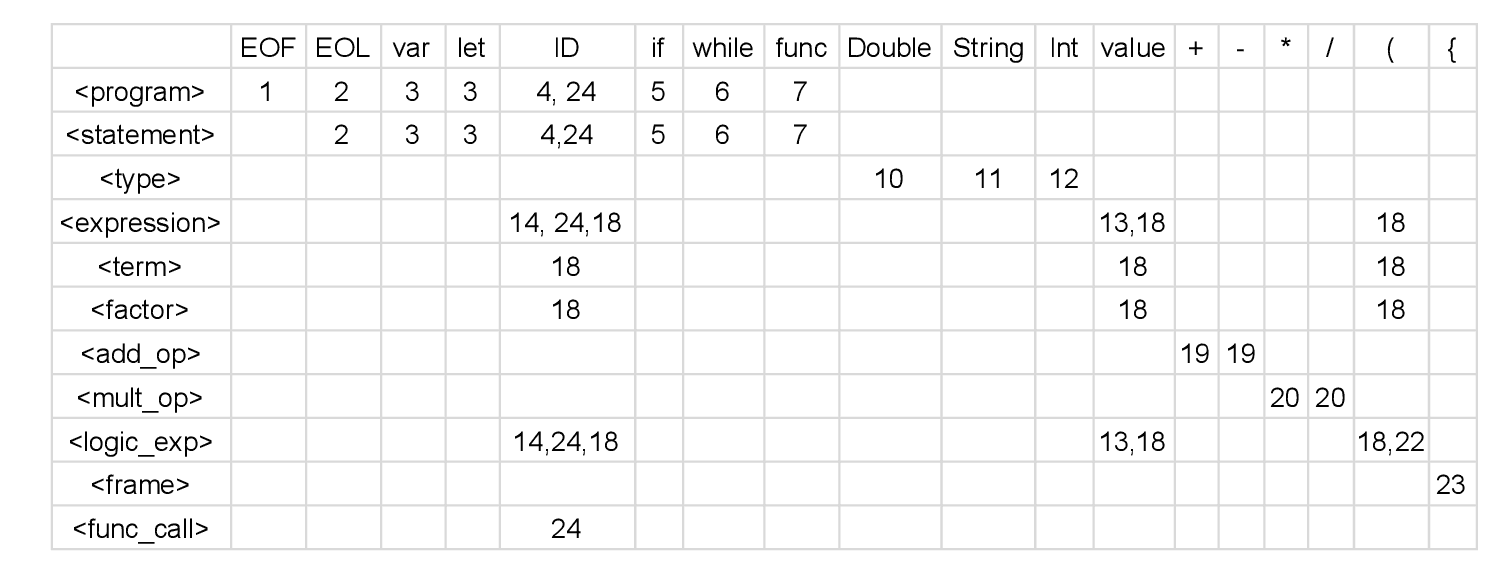
\includegraphics[width=1\linewidth]{inc/LL_table.pdf}
		\caption{LL -- tabulka použitá při syntaktické analýze}
		\label{table:ll_table}
	\end{table}


	\subsection{Precedenční tabulka}
	\begin{table}[!ht]
		\centering
		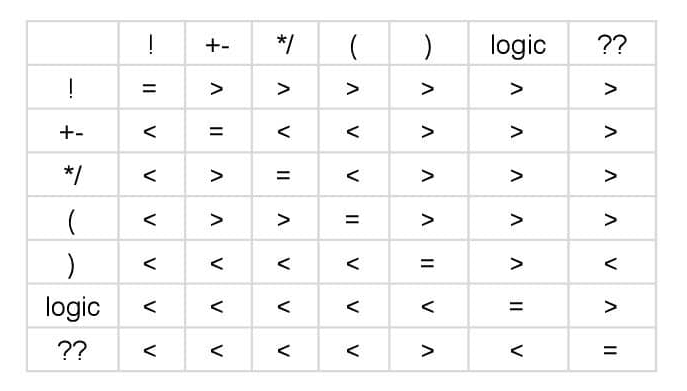
\includegraphics[width=0.7\linewidth]{inc/prec_table.pdf}
		\caption{Precedenční tabulka použitá při precedenční syntaktické analýze výrazů}
		\label{table:prec_table}
	\end{table}


\end{document}
